\documentclass[fr]{../../../eplsummary}

\usepackage{../../../eplmath}
\usepackage{float}

\graphicspath{{img/}}

\newcommand{\Cmn}{\C^{m \times n}}
\newcommand{\Cmm}{\C^{m \times m}}
\newcommand{\Cn}{\C^{n}}
\newcommand{\Cm}{\C^{m}}
\renewcommand{\ker}{\ensuremath{\mathrm{null}}}
\newcommand{\colsp}{\ensuremath{\mathrm{range}}}
\newcommand{\rank}{\ensuremath{\mathrm{rank}}}
\newcommand{\adj}[1]{{#1}^{*}}
\DeclarePairedDelimiterX{\inp}[2]{\langle}{\rangle}{#1, #2}

\hypertitle[']{Analyse numérique}{5}{INMA}{1170}
{Gilles Peiffer}
{François Henrotte et Jean-François Remacle}

\section{Bases d'algèbre linéaire}
L'algèbre linéaire est l'étude de l'équation
\[
Ax = b\,.
\]
Il y a quatre façons de voir cette équation:
\begin{enumerate}
	\item Comme un \emph{produit matrice-vecteur}, où
	\[
	A \in \Cmn\,, \quad x \in \Cn\,, \quad b \in \Cn\,.
	\]
	\item Comme une \emph{expression tensorielle}:
	\[
	b_i = \sum_{j=1}^{n} a_{ij}x_i\,,
	\]
	où $a_{ij}$ est l'entrée
	à la $i$\ieme{} ligne
	et la $j$\ieme{} colonne de $A$.
	\item Comme disant que
	\emph{$b$ est dans le \textbf{column space} de $A$}\footnote{Espace vectoriel sous-tendu par les colonnes de $A$.},
	et est donc une combinaison linéaire des colonnes de $A$.
	\[
	b = Ax = \sum_{j=1}^{n} x_j a_j\,,
	\]
	où $a_j$ est la $j$\ieme{} colonne de $A$.
	\item Comme une \emph{application linéaire} de $\Cn$ dans $\Cm$:
	\[
	A \colon \Cn \to \Cm\,.
	\]
	On a donc les propriétés suivantes:
	\[
	\begin{array}{rcl@{\quad}l}
		A(x+y) & = & A(x) + A(y)\,, & \quad \forall x,y \in \Cn\,,\\
		A(\alpha x) & = & \alpha A(x)\,, & \quad \forall x \in \Cn\,,
		\quad \alpha \in \C\,.
	\end{array}
	\]
\end{enumerate}

\subsection{Produit matrice-matrice}
Le produit matrice-matrice
\[
B = AC\,, \quad B \in \C^{l \times n}\,,\quad A \in \C^{l \times m}\,,\quad C \in \Cmn
\]
est une généralisation du produit matrice-vecteur vu précédemment.
On peut également l'écrire
\begin{align*}
	b_{ij} &= \sum_{k=1}^{m} a_{ik}c_{kj}\,.
\end{align*}
Chaque colonne de $B$ est une combinaison linéaire
des colonnes de $A$.

\subsection{Définitions}
\begin{mydef}[Column space]
	Le \emph{column space} d'une matrice $A \in \Cmn$,
	également noté $\colsp(A)$ est défini comme
	\[
	\colsp(A) = \mathrm{span}\{a_1, a_2, a_3, \dots, a_n\}\,.
	\]
\end{mydef}
\bigbreak
\begin{mydef}[Kernel]
	Le \emph{kernel} (\emph{noyau}, encore appelé \emph{null space}) d'une matrice $A \in \Cmn$
	est défini comme
	\[
	\ker(A) = \set{x \in \Cn \suchthat Ax = 0}\,.
	\]
	Les composantes de chaque vecteur de $\ker(A)$
	sont les coefficients d'une combinaison linéaire nulle
	des colonnes de $A$.
	\[
	Ax = 0 \iff \sum_{j=1}^{n} x_j a_j = 0\,.
	\]
\end{mydef}
\bigbreak
\begin{mydef}[Rang]
	Le \emph{rang} d'une matrice $A \in \Cmn$
	est défini comme la dimension de $\colsp(A)$:
	\[
	\rank(A) = \dim(\colsp(A))\,.
	\]
	Les espaces vectoriels sous-tendus
	par les lignes et les colonnes d'une matrice (carrée ou rectangulaire)
	ont toujours la même dimension.
	On appelle rang de la matrice $A$ cette dimension.
	On a donc nécessairement
	\[
	\rank(A) \le \min(m,n)\,.
	\]

	On dit qu'une matrice est \emph{de plein rang} lorsque
	\[
	\rank(A) = \min(m,n)\,.
	\]
	Une matrice est de plein rang si et seulement si
	jamais deux vecteurs différents de son domaine n'ont la même image.
	Cela implique que l'application
	\[
	A \colon \Cn \to \colsp(A) \subseteq \Cm
	\]
	est bijective\footnote{La démonstration est en page 7 du livre.}.
	% TODO add bib reference, maybe put this in an appendix?

	Il n'y a qu'une seule matrice \emph{de rang zéro} par dimension:
	la matrice nulle.

	Pour ce qui en est des matrices \emph{de rang un},
	prenons les vecteurs suivants:
	\begin{align*}
		u &\in \C^{m \times 1}\,,\\
		v &\in \C^{1 \times n}\,.
	\end{align*}
	Leur produit s'écrit
	\[
	\big(uv\big)_{ij} = u_i v_j\,.
	\]
	Cette matrice $\big(uv\big)_{ij}$ est de rang un,
	car toutes ses colonnes sont multiples de $u$.
\end{mydef}
\bigbreak
\begin{mydef}[Matrice inversible]
	Une matrice carrée $A \in \Cmm$ est \emph{inversible}
	si elle satisfait les propositions ci-dessous.
	Toutes les propositions suivantes sont équivalentes:
	\begin{enumerate}[label=(\alph*)]
		\item $A$ est inversible;
		\item $\rank(A) = m$ ($A$ est de plein rang);
		\item $\colsp(A) = \Cm$;
		\item $\ker(A) = \{0\}$ (et \emph{non pas} $\emptyset$);
		\item $0$ n'est pas une valeur propre de $A$;
		\item $0$ n'est pas une valeur singulière de $A$;
		\item $\det(A) \ne 0$.
	\end{enumerate}
\end{mydef}
\bigbreak
\begin{mydef}[Matrice adjointe]
	Si $A \in \Cmn$, la \emph{matrice adjointe} de $A$,
	notée\footnote{Une autre notation possible est $A^{\dag}$.} $\adj{A}$,
	est la matrice obtenue:
	\begin{itemize}
		\item en prenant le complexe conjugué de chaque coefficient;
		\item en permutant lignes et colonnes.
	\end{itemize}
	Remarquons que si $A$ est réelle, $\adj{A} = A^T$.
\end{mydef}
\subsection{Produit scalaire}
Un \emph{produit scalaire} (ou \emph{produit intérieur})
est une opération bilinéaire
\[
\inp{\cdot}{\cdot} \colon \Cm \times \Cm \to \C
\]
telle que
\[
\inp{\adj{x}}{y} = \sum_{i=1}^{m} \widebar{x_i} y_i\,,
\]
où $\widebar{x_i}$ est le complexe conjugué de $x_i$.

Reprenons nos vecteurs $u \in \C^{1 \times m}$
et $v \in \C^{m \times 1}$.
On a que
\[
\inp{u}{v} = \sum_{i=1}^{m} u_i v_i\,.
\]
Comme l'opération est bilinéaire,
on a
\[
\renewcommand{\arraystretch}{1.5}
\begin{array}{rcl@{\quad}l}
	\inp[\big]{\adj{\big(x_1 + x_2\big)}}{y} & = & \inp{\adj{x_1}}{y} + \inp{\adj{x_2}}{y}\,, & \forall x_1, x_2, y \in \Cm\,,\\
	\inp[\big]{\adj{x}}{\big(y_1 + y_2\big)} & = & \inp{\adj{x}}{y_1} + \inp{\adj{x}}{y_2}\,, & \forall x, y_1, y_2 \in \Cm\,,\\
	\inp[\big]{\adj{\big(ax\big)}}{by} & = & \widebar{a}b\inp{\adj{x}}{y}\,, & \forall a,b \in \C\,, \quad \forall x,y \in \Cm\,.
\end{array}
\]
\subsubsection{Longueur d'un vecteur}
Avec ce produit scalaire,
il est possible de définir la longueur d'un vecteur:
\[
\norm{x} = \sqrt{\inp{\adj{x}}{x}}\,, \quad \textnormal{si } x\in \R^{m}\,.
\]

\subsubsection{Angle entre deux vecteurs}
Le produit scalaire permet aussi
de définir l'angle entre deux vecteurs:
\[
\cos \alpha = \frac{\inp{\adj{x}}{y}}{\norm{x}\norm{y}}\,.
\]
\subsubsection{Orthogonalité}
Grâce au produit scalaire,
on peut définir le concept d'orthogonalité
\begin{itemize}
	\item de deux vecteurs:
	\[
	\inp{\adj{x}}{y} = 0 \iff \inp{\adj{y}}{x} = 0\,,
	\]
	\item d'un ensemble $\mathcal{S}$ de vecteurs:
	\[
	\inp{\adj{x}}{y} = 0\,, \quad \forall x,y \in \mathcal{S} \suchthat x \ne y \implies \textnormal{ils sont linéairement indépendants,}
	\]
	\item de deux ensembles $\mathcal{S}$ et $\mathcal{S}'$
	de vecteurs non nuls:
	\[
	\inp{\adj{x}}{y} = 0\,,\quad \forall x \in \mathcal{S}\,,\quad \forall y \in \mathcal{S}'\,.
	\]
\end{itemize}
\subsubsection{Décomposition orthogonale}
Soit un ensemble $\mathcal{Q} = \{q_1,q_2,\dots,q_n\}$ de vecteurs orthonormés
formant une base orthonormée
pour un sous-espace de dimension $n \le m$ de $\Cm$.
On a alors\footnote{Où $\delta_{ij}$ est le \emph{symbole de Kronecker}.}
\[
\inp{\adj{q_i}}{q_j} = \delta_{ij}\,,\quad i,j = 1,\dots,n\,.
\]
Soit $v \in \Cm$.
On a la décomposition orthogonale
\begin{align*}
v &= r + \sum_{i=1}^{n} \inp{\adj{q_i}}{v} q_i\\
&= r + \sum_{i=1}^{n} \inp{q_i}{\adj{q_i}} v\,,
\end{align*}
avec $\inp{\adj{q_i}}{r} = 0$,
c'est-à-dire $r \perp \mathcal{Q}$.
\subsubsection{Matrice unitaire}
Une matrice unitaire est une matrice carrée vérifiant
\[
\adj{Q} = Q^{-1} \iff \adj{Q}Q = I\,,
\]
qui s'écrit également
\[
\inp{\adj{q_1}}{q_2} = \delta_{ij}\,,
\]
en termes des colonnes de $Q$.
Les colonnes d'une matrice unitaire de $\Cmm$
forment une base orthonormée pour $\Cm$.
\subsubsection{Isométrie}
Une matrice unitaire laisse le produit scalaire invariant:
\[
\inp[\big]{\adj{\big(Qx\big)}}{Qy} = \inp{\adj{x}}{y}\,.
\]
Les longueurs des vecteurs et les angles qu'ils forment
sont donc également invariants\footnote{En mécanique des solides déformables,
cela donne lieu aux rotations et aux réflexions
selon que $\det(Q)$ soit $1$ ou $-1$ respectivement.}.
\subsection{Normes vectorielles}
Une norme vectorielle est une fonction
\[
\norm{\cdot} \colon \Cn \to \R
\]
satisfaisant les trois hypothèses suivantes:
\begin{itemize}
	\item \emph{séparation}: $\norm{x} \ge 0$
	avec l'égalité si et seulement si $x = 0$;
	\item \emph{inégalité triangulaire}: $\norm{x+y} \le \norm{x} + \norm{y}$;
	\item \emph{homogénéité absolue}: $\norm{ax} = \abs{a}\norm{x}\,,\quad \forall a \in \C$.
\end{itemize}

\begin{myrem}
	\emph{Le produit scalaire n'est donc pas une norme},
	car il ne satisfait pas la deuxième hypothèse.
	Cependant, sa racine carrée l'est.
\end{myrem}

Il existe beaucoup de normes différentes,
comme par exemple les $p$-normes(ou $\ell^p$-normes):
\begin{itemize}
	\item la norme $\ell^1$ définie par
	\[
	\norm{x}_1 \coloneqq \sum_i \abs{x_i}\,;
	\]
	\item la norme $\ell^2$ définie par
	\[
	\norm{x}_2 \coloneqq \sqrt{\sum_i x_i^2}\,;
	\]
	\item la norme $\ell^p$ définie par
	\[
	\norm{x}_p \coloneqq \left(\sum_i \abs{x_i}^p\right)^{1/p}\,;
	\]
	\item la norme $\ell^{\infty}$ définie par
	\[
	\norm{x}_\infty \coloneqq \max_i \abs{x_i}\,.
	\]
\end{itemize}
On peut donner une représentation graphique de ces normes vectorielles.
On définit pour cela les \emph{boules unitaires} (\emph{unit balls}):
\[
B_p^m = \set[\big]{x \in \Cm \suchthat \norm{x}_p \le 1}\,.
\]
\begin{figure}[H]
	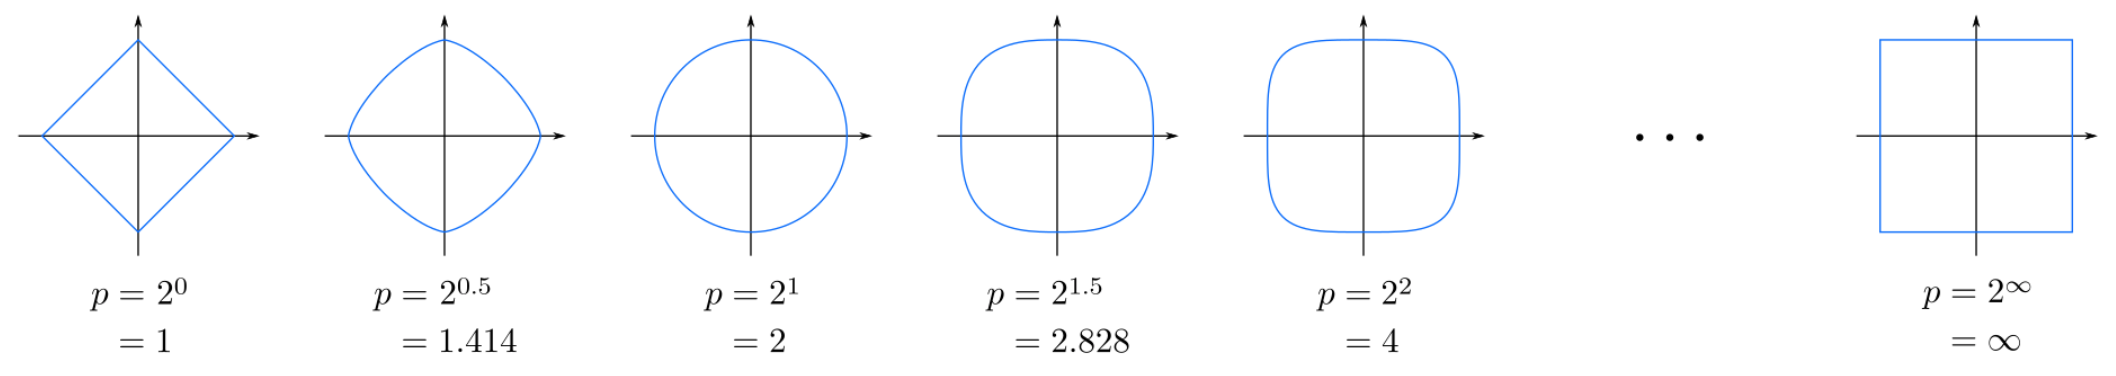
\includegraphics[width=\textwidth]{unit_balls.png}
	\caption{Une visualisation des boules $B_p^1$ pour $p \in \intervalco{1}{+\infty}$.}
	\label{fig:unit_balls}
	% TODO bib ref (wikipedia; unit ball)
\end{figure}
Comme on le voit sur la figure,
\[
B_p^m \subsetneq B_q^m\,,\quad \forall p < q\,.
\]
\subsection{Norme matricielle}
La norme matricielle induite par une norme vectorielle
est une norme pour les matrices
regardées comme des opérateurs sur les vecteurs.
Soit $A \in \Cmn$ un opérateur $A \colon \Cn \to \Cm$
et $\norm{\cdot}_{(m)}$ et $\norm{\cdot}_{(n)}$ deux normes vectorielles
respectivement sur $\Cm$ et $\Cn$.
On définit la norme matricielle $\norm{\cdot}_{(m,n)}$
induite par ces normes vectorielles par
\[
\norm{A}_{(m,n)} \coloneqq \sup_{x \in \Cn \setminus \{0\}} \frac{\norm{Ax}_{(m)}}{\norm{x}_{(n)}}\,.
\]
Comme toute norme doit satisfaire l'hypothèse d'homogénéité absolue,
et que $A$ est linéaire,
on voit que la norme de $x$ n'intervient pas dans la norme matricielle.
On peut également définir cette norme sans division:
\[
\norm{A}_{(m,n)} \coloneqq \sup_{x \in B_p^m} \norm{Ax}_{(m)}\,.
\]
\end{document}
